\documentclass[../report.tex]{subfiles}
\begin{document}
% --------------------------------------------------------------------------
% SECTION 3 
% --------------------------------------------------------------------------
\section{System Identification}

\textbf{System name:} Helicopter azimuth \\
\textbf{List of files:} 
\begin{tabular}{ |c|c| }
    \hline
    measure.m & Script for measuring I/O data \\
    main\_params\_plot.m & Define parameters and plot data \\
    model\_data\_measure.slx & Model for data measurement \\
    model.slx & Main model \\
    model\_simple.slx & Simplify model \\
    heli\_data.mat & Measured data for parameter estimation \\
    model\_estimation\_session.mat & Parameter estimation session \\
    \hline
\end{tabular} \\

\subsection{System analysis and generation I/O data}

The following Simulink model was used to measure the data
\ref{fig:data_measure}
\begin{figure}[htb!]
    \centering
    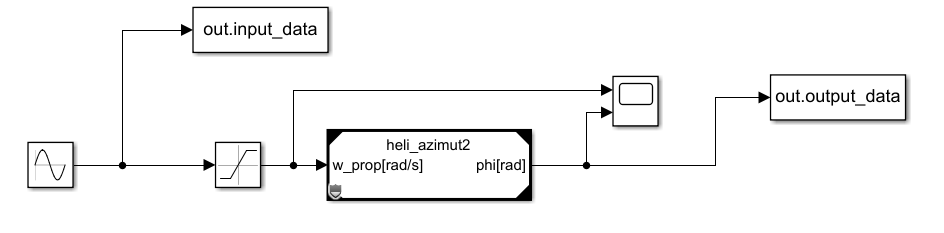
\includegraphics[width=0.8\textwidth]{data_measure.png}
    \caption{Simulink model for data measurement}
    \label{fig:data_measure}
\end{figure}

3 types of input data were used: sine function, step response, pulse
function \ref{fig:ident_data_1}.

\begin{figure}[htb!]
    \centering
    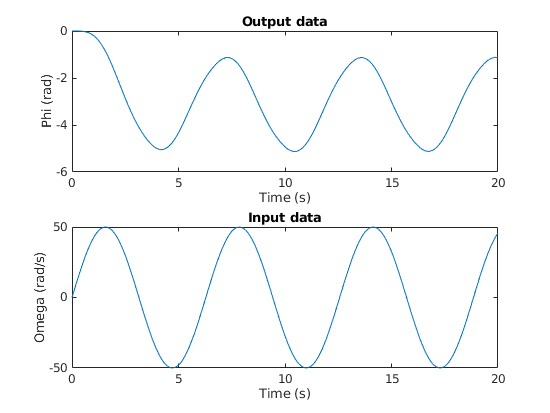
\includegraphics[width=0.6\textwidth]{ident_data_1.png}
    \caption{Simulink model for data measurement}
    \label{fig:ident_data_1}
\end{figure}
\begin{figure}[htb!]
    \centering
    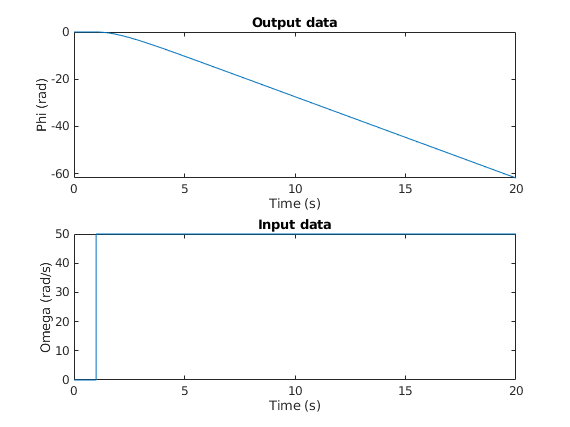
\includegraphics[width=0.6\textwidth]{ident_data_2.png}
    \caption{Simulink model for data measurement}
    \label{fig:ident_data_2}
\end{figure}
\begin{figure}[htb!]
    \centering
    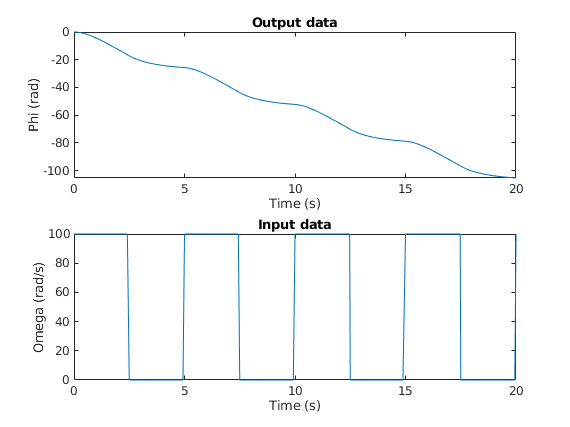
\includegraphics[width=0.6\textwidth]{ident_data_3.png}
    \caption{Simulink model for data measurement}
    \label{fig:ident_data_3}
\end{figure}

\subsection{Model description}

\begin{tabular}{ |c|c| }
    \hline
    $a$ & Side length of flat plate perpendicular to flow [$m$]\\
    $\theta$ & Turn angle [$rad$]\\
    $m$ & Mass [$kg$]\\
    $\omega$ & Angular velocity of propeller [$rad/s$]\\
    $L$ & Length [$m$]\\
    $I$ & Moment of inertia [$kg/m^2$]\\
    $b$ & Friction coefficient [-]\\
    $C_x \approx 1.28$ & Drag coefficient [-]\\
    $\rho \approx 1.2$ & Mass density of the fluid [$kg/m^3$]\\
    $A$ & Propeller area [$m^2$]\\
    $S = a^2$ & Area of flat plate [$m^2$] \\
    \hline
\end{tabular} \\

\begin{figure}[htb!]
    \centering
    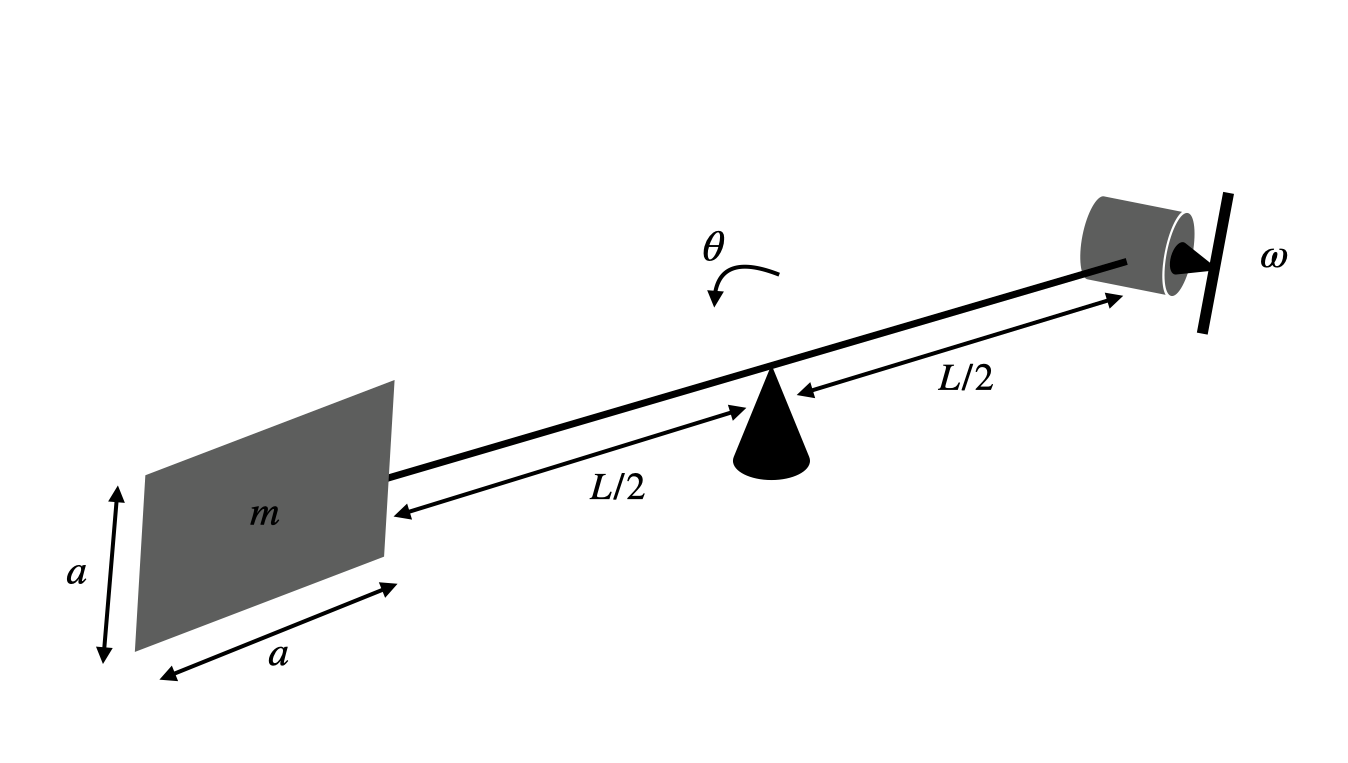
\includegraphics[width=0.6\textwidth]{ident_model.png}
    \caption{Model helicopter azimuth}
    \label{fig:ident_model}
\end{figure}
Math model of helicopter azimuth described by equation \ref{math_model_eq}.

\begin{equation}
    I\ddot{\theta} = M_{prop} - (M_f + M_d)
\end{equation}
$M_d = \frac{1}{2}C_x \rho S \left(\frac{L}{2}\right)^3\dot{\theta}^2$ -  
drag equation.\\
$M_f =  b\dot{\theta}$ - friction momentum. \\
$M_p = \frac{\rho AL}{4}\omega^2$ - momentum from propeller thrust.


\begin{equation}\label{math_model_eq}
    \ddot{\theta} = \frac{\rho AL}{4I}\omega^2 - \frac{b}{I}\dot{\theta}
    - \frac{1}{2I}C_x \rho S \left(\frac{L}{2}\right)^3\dot{\theta}^2 
\end{equation}

Parameters to estimation:
$p_0 = \frac{AL}{I}$, $p_1 = \frac{b}{I}$, $p_2 = \frac{SL^3}{I}$


Simulink model represented in following diagram
\ref{fig:ident_model_simulink_full}.
\begin{figure}[htb!]
    \centering
    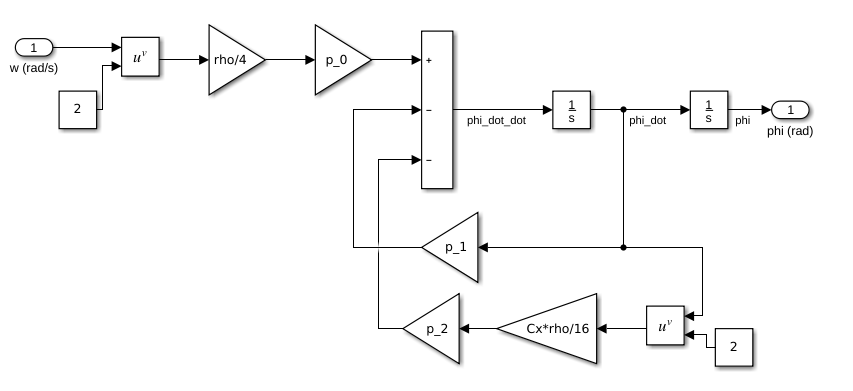
\includegraphics[width=0.8\textwidth]{ident_model_simulink_full.png}
    \caption{Simulink model of helicopter azimuth}
    \label{fig:ident_model_simulink_full}
\end{figure}

\subsection{Parameter estimation}

The model \ref{fig:ident_model_simulink_full} doesn't working with
Parameter Estimation App. The problem is power variables. That's why I was
forced to remove powers and simplify a model to
\ref{fig:ident_model_simulink}.
\begin{figure}[htb!]
    \centering
    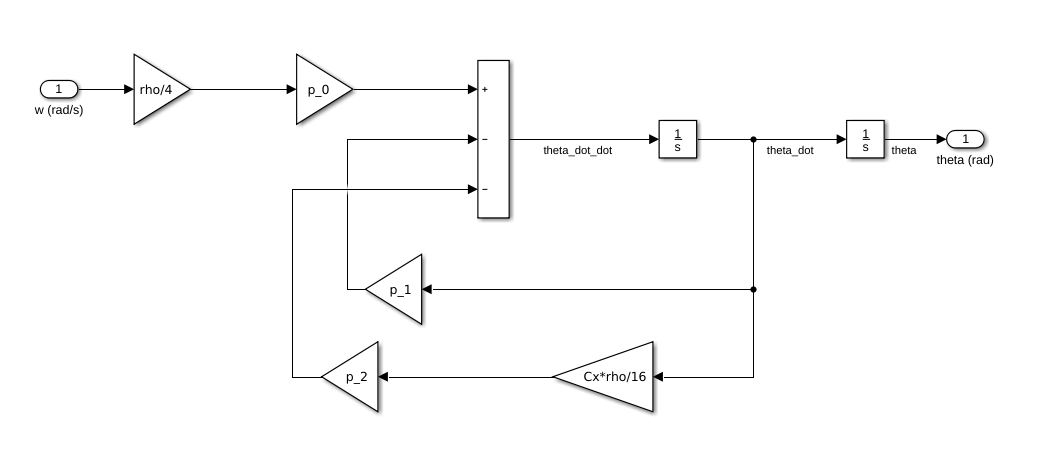
\includegraphics[width=0.8\textwidth]{ident_model_simulink.png}
    \caption{Simulink simplify model of helicopter azimuth}
    \label{fig:ident_model_simulink}
\end{figure}

The results are saved and can be checked in \textbf{model\_estimation\_session.mat}.

\subsection{Feed-forward}
\subsection{System Identification (Black-box)}
\subsection{Evaluation of the whole task and conclusion}
The parameter estimation app did not work with powers of the parameters,
therefore the model was simplified from \ref{fig:ident_model_simulink_full} to
\ref{fig:ident_model_simulink}. Estimation approached the output
data but not exactly. 

\end{document}
